\documentclass[a4paper]{IEEEtran}
\usepackage[top=2.5cm, bottom=3cm, left=2.cm, right=2.cm]{geometry}
\usepackage[utf8]{inputenc}
\usepackage[english]{babel}
%\usepackage{amsmath}
\usepackage{amsmath}
\usepackage{bm}
\usepackage{graphicx}
\usepackage{caption}
\usepackage{subcaption}
%\usepackage{subfig}
\usepackage{array}
\usepackage[thinlines]{easytable}
\usepackage[export]{adjustbox}
\usepackage{pseudocode}
\usepackage{wrapfig}
\usepackage[backend=bibtex, style=ieee]{biblatex}
\usepackage{xcolor}
\usepackage[]{rotating}
\usepackage[]{titlesec}
\usepackage[absolute]{textpos}
\usepackage{footnote}
\usepackage{pdflscape}
\usepackage{pgfgantt}
%\usepackage[tocflat]{tocstyle}
\usepackage{multicol}
\usepackage{diagbox}
\usepackage{lipsum}
\usepackage[multiple]{footmisc}

\makesavenoteenv{tabular}
\makesavenoteenv{table}

\definecolor{themecolor}{RGB}{80, 0, 127} %manchester
\definecolor{themecolordark}{RGB}{64, 26, 86} %dark-manchester
\definecolor{darkgray}{gray}{0.15}


\addbibresource{mybibliography.bib}

\graphicspath{{./images/}}


%opening

%\titleformat{\section}[hang]{\color{black}\large\sffamily\bfseries}{\thesection.}{0.4em}{\vspace*{-6pt}}
%\titleformat{\subsection}[hang]{\color{black}\normalsize\sffamily\bfseries}{}{0pt}{\vspace*{-4pt}}
%\titleformat{\subsubsection}[hang]{\color{black}\normalsize\sffamily\itshape}{}{0pt}{}

%\title{Computer Vision on the SpiNNaker Platform}
\title{Real-Time Implementation of Retinal Models}
\author{Garibaldi Pineda Garc\'ia\\
        Supervisor: Steve Furber, Co-Supervisor: Dave Lester\\
        School of Computer Science, University of Manchester, U.K.}
\date{}


\begin{document}
\pagenumbering{gobble}
\thispagestyle{empty}
%\setlength{\TPHorizModule}{1mm}
\setlength{\TPVertModule}{1mm}
\begin{titlepage}
  ~
  \begin{textblock}{50}(175,0)
    \begin{color}{themecolor}
      \rule{3cm}{30cm}
    \end{color}
  \end{textblock}

  \begin{textblock}{160}(-10,33)
    \begin{color}{themecolor}
      \rule{160cm}{2.2cm}
    \end{color}
  \end{textblock}
  
  % Logo white
  \begin{textblock}{150}(20,30)
    \begin{flushright}
    %\rule{2cm}{2cm}\\[2em]   
    
\includegraphics[height=20mm]{manchester-logo}\\[5em]
    
    {\noindent\Huge\bfseries SpiNNaker-based Visual Systems}\\[2em]
    
    {\noindent\huge End-of-first-year report }\\[5em]
    
    {\noindent\Large\bfseries Garibaldi~Pineda~García}\\[0.5em]
    {\noindent\Large Supervisor: Steve~Furber}\\[0.1em]
    {\noindent\Large Co-supervisor: Dave~Lester}\\[1em]
    {\noindent\large Advanced Processing Technologies Group\\
      School of Computer Science \\
      University of Manchester\\[0.4em]
      United Kingdom}
    \end{flushright}
  \end{textblock}
  
  
  \begin{textblock}{20}(186,285)
    \begin{rotate}{90}
      %{\huge\sffamily\bfseries \textcolor{white}{University of Manchester}}
      {\huge\bfseries \textcolor{white}{University of Manchester}}
    \end{rotate}
  \end{textblock}
  \begin{textblock}{20}(196,285)
    \begin{rotate}{90}
      %{\huge\sffamily\bfseries \textcolor{white}{University of Manchester}}
      {\huge\bfseries \textcolor{white}{APT Group}}
    \end{rotate}
  \end{textblock}  

  \begin{textblock}{150}(20, 250)
    \begin{flushright}
    
\includegraphics[height=30mm]{spinnaker-logo}
    \end{flushright}
  \end{textblock}
  
\end{titlepage}
\maketitle
%\newpage

%\tableofcontents
%\vspace*{1em}
\pagenumbering{arabic}

%\section*{Abstract}
\begin{abstract}
Vision systems in biological entities are among the most complex sensory
inputs in nature. If we want to simulate them, it would require incredible
amounts of computing power and, traditionally, several algorithms to perform
each individual task. A parallel computation platform is the best way to go
while attempting to solve this problem, since neural structures in the brain 
compute in this way. 

SpiNNaker is one of such platforms, a network of low-powered processing units,
each of which can simulate several neurons. Given that the SpiNNaker platform
resembles this natural neural structures, computer vision algorithms need to be
developed in a completely different manner.

The aim of this project is to develop algorithms in the realm of computer vision
but using a spiking neural networks approach. In particular we'll study 
time-based spike codes and how to process them. This algorithms should be 
able to cooperate and share their interpretation of the input data to gain a
more robust understanding of images.

\end{abstract}

\section{Introduction}
\label{sec-intro}
For most animals, an important part of perception is done through visual input.

This kind of input has given humans the possibility of culture through reading and writing, cognitive development.

We might take vision for granted, but we are reminded of its importance when we hear an unusual noise in a dark room. 

An important aspect of vision is our ability to create mental maps of our current or, even past, locations.

The goal of the project is to create a 3D environment reconstruction.

There has been work on this field on ``classic'' computer vision, but for real-time they rely on high-performance power-hungry devices. Something that limits the actual utility of such systems for mobile applications. It would be a bit inconvenient to carry around a couple of car batteries in ones pocket.

We are able to do it with a highly-parallel 20-watts neural blob. There must be a more efficient way of doing this. A brief description of the brain and its function can be found in Chapter \ref{chp:brain}. We delve into the components of human vision in Chapter \ref{chp:vision}.

SpiNNaker provides a massively-parallel high-efficiency computing platform, inspired by the brain. It's an excellent choice for neuroscience research, particularly to study spiking neural networks. Its software stack has many ready-to-use neural models and development of new models can be performed in a straight forward manner. Chapter \ref{chp:neuro-hw} has a more detailed description of this and other neuromorphic hardware.\\


Input for spiking neural networks has to be in \emph{spike trains}, which are a series of spikes emitted by a neuron in a given time slot. In order to use video sources they need conversion. Few solutions which, mostly, require the use of custom hardware which is expensive and has low availability. We propose a parallel software based encoding.

This years work consisted in creating an input system for our spiking neural networks; details of this can be found in Chapter \ref{chp:img2spk}. 

While there are some examples of hardware based retinas, they are still expensive or they have limited availability. Implementing a retina model using consumer hardware is of great help for people that are unable to obtain a silicon retina.

Of special interest are mobile applications, if we can provide a low-power solution to a silicon retina emulator, we could enable millions of phones, tablets or computers to work as an input to neural computations (QUALCOMM CHIP, SPINNAKER) and keep the traditional camera functionality.

\section{Problem description}
\label{sec:intro:problem}
Environment reconstruction is an active field of research, particularly from the Simultaneous Localization and Mapping (SLAM) community\cite{Thrun2008_SLAM}. \textbf{SMALL DESCRIPTION OF SLAM!!!} 
%GPS unreliable because it's not precise, a couple of meters of difference could lead a car jumping on the curve or bumping another while trying to park.

Humans are able to do something similar with an efficient highly-parallel neural computing system that requires about 20-watts to function. How exactly this is done in the brain is still an open question. This research will provide a solution, inspired by state-of-the-art neuroscience, to the environment reconstruction problem using neuromorphic hardware.

Most research has cameras and a mixture of exotic depth sensors as inputs. One implication of this type of input is large quantities of information having to be processed, thus, needing high-performance and power-hungry devices to execute their algorithms. This is something that limits the actual utility of such systems for mobile applications. On the other hand, neuromorphic sensors have shown to reduce representations so that irrelevant information is not transmitted nor processed~\cite{aer-retina-bernabe,dvs-zurich}.

Another disadvantage to using ``classic'' computer vision approaches is that computational resources would need to be shared inefficiently (i.e. a processor would have to switch between a facial recognition algorithm to a depth-estimation one). Having a neuro inspired system means that the tasks are executed by the same network.

SpiNNaker provides a massively-parallel high-efficiency computing platform, inspired by the brain. It's an excellent choice for neuroscience research, particularly to study spiking neural networks. Its software stack has many ready-to-use neuron models and development can be performed in a straight forward manner~\cite{furber2014spinnaker}. 



\section{Objectives}
\label{sec:intro:objectives}
3D environment reconstruction is a very active field of research.
Advances in depth perception (KINECT) have made real-time simultaneous localization and mapping (SLAM) a possibility.
One way of achieving is to use high-performance GPUs and solve the problem using raw power.
Another is to use a mix of KINECT and RETINA, not fully neural???
We propose using an exclusively neural networks approach using SpiNNaker hardware.
\section{Plan}
\label{sec:intro:plan}
Steps:
\subsection{Image recognition}
\label{subsec:intro:plan:2D-recognition}
Time-based encoding, learning, classification, deep belief networks comparison, hierarchical structures

\subsection{3D object recognition}
\label{subsec:intro:plan:3D-recognition}
Correlation in space and time, spiking neural networks should make an excellent match for this.

\subsection{Depth perception}
\label{subsec:intro:plan:depth-perception}
Binocular, depth-from-defocus, other sensors? Optic flow to infer motion?

\subsection{Orientation and localization}
\label{subsec:intro:plan:localization}
Even more sensors? Make statistics/probabilistic models of past data?

\subsection{Reconstruction}
\label{subsec:intro:plan:reconstruction}
Get a top down approach? Interface 2 nets?


\section{Research Aims and Contribution}
\label{sec-aims-contribs}
This research aims to develop computer vision algorithms using SpiNNaker. This 
is to be achieved by modelling biological vision, using spiking neural networks,
on SpiNNaker. Several stages of vision would need modelling and/or 
implementation, the latter has been the goal for this year's work.
We hypothesize that a better understanding of vision in biology will lead to 
a unified computer vision framework. Using neural networks should translate in 
gaining an insight to the meaning of elements in a scene and, thus, a relation
between different images of the same scenario.

Bio-inspired vision algorithms using SpiNNaker hardware could be used on 
robotics, security or transportation applications. The research on learning and 
classification could lead into a theory of learning and memory in the brain.

\section{Previous Work}
\label{sec-prev-work}
In order to process visual input from frame based imaging devices on a spiking 
neural network (SNN) a transformation is needed. The most common way is to 
simply encode using Poisson spiking with a rate that is proportional to pixel
intensity. This is just modelling the photoreceptor layer in the retina as 
other cell layers react to changes in intensity\cite{webvision} and perform 
other computation before emitting actual spikes. One of the most accurate 
retinal models was developed by \citeauthor{virtual-retina} in 
\cite{virtual-retina}. A special category is hardware based bio-inspired 
retinas. First reported on \cite{carver-mead}. New devices have been developed 
and reported in \cite{aer-retina-bernabe, dvs-zurich}, this are splendid 
real-time, low-powered, high-dynamic-range event-based cameras; though they 
have limited availability.



\section{Project Progress to Date}
\label{sec-project-progress}
The literature review is about 60\%, though further reading might prove that 
this number might change. 
Converting DVS emu
Converting BASAB model GPU, SPINNAKER, video transfer
Paper on MNIST

%
%Converting frame-based video into spike-trains is a computationally 
%intensive and time consuming task. There are very few equipment that can
%produce spikes from video and they are either in development or too expensive,
%thus every-day users are put behind a virtual wall, leaving them unable to
%experiment with visual input in their simulations or robotics applications. An
%efficient parallel implementation of a simple yet powerful retinal model would
%remove this wall by reducing the time it takes to compute a spike
%representation of a video frame. Furthermore if this is done on
%consumer graphics processing hardware, it will allow almost any user to
%generate their own spike-trains.
%
%In most animals the eye is the organ that captures light so that it can be
%processed in the retina and sent further down the brain as multiple spike
%trains (section \ref{sec-retina}). The retina has been modelled using different
%approaches that go from the extremely detailed (i.e. cell-by-cell)
%\cite{virtual-retina} to the functional
%\cite{basab-model,thorpe-spike-rapid-processing}. We have chosen what we
%believe to be the best model for real-time video processing (section
%\ref{sec-fov-pit}). This model provides a simple and elegant solution to
%encoding, though it suffers from redundancy issues, which are alleviated using
%further processing.
%
%Later in this work we present different strategies to achieve real-time
%encoding into spike trains of video with higher resolution (section
%\ref{sec-parallel}) exploiting the parallelism that comes with image
%processing. To verify that our spike train sets are correct, we test them using
%a reconstruction procedure (section \ref{sec-reconstruction}).



\section{Thesis Outline}
\label{sec-thesis-toc}
%\begin{multicols}{2}
  \begin{itemize}
      \item Abstract
      \item \textbf{Chapter 1}. Introduction.
      \begin{itemize}
        \item Neural networks.
        \item Spike codes in vision.
        \item Inhibition.
        \item Spatio-temporal patterns and learning.
        \item Research objectives.
      \end{itemize}
      \item \textbf{Chapter 2}. Background.
      \begin{itemize}
        \item SpiNNaker platform.
        \item Real-time artificial neural computations.
        \item Polychronization.
        \item Classification.
      \end{itemize}
      \item \textbf{Chapter 3}. Methodology.
      \begin{itemize}
      \item Model visual input using time-based spike codes.
      \item Hierarchical networks for robust classification.
      \item Feature identification.
      \item Sensor fusion and image registration.
      \end{itemize}
      \item \textbf{Chapter 4}. Results.
      \begin{itemize}
        \item Comparison with other methods.
        \item Discussion.
      \end{itemize}
      \item \textbf{Chapter 5}. Conclusions and Further Work.
      \begin{itemize}
        \item Conclusions.
        \item Future work.
        \item Publications.
      \end{itemize}
      \item \textbf{References}.
      
  \end{itemize}
%\end{multicols}

\section{Conclusions and further work}
\label{sec-conclusions}
A complete model the visual cortex remains an open research question. Though many neural networks and computer vision models account for single visual functions, a unified solution has not been developed. Since environment reconstruction makes use of many of these functions, this research could lead to contributions to a general theory of vision. 

A hierarchical neural networks approach promises to have better results. The training of deep spiking neural networks is still in early stages of research, which brings another opportunity for contributions to neuroscience. Recurrent neural networks could provide the necessary framework to solve the training problem.

\section{Publications}
\label{sec-publications}
Part of the work carried during this year will be published as a paper on a 
\textbf{Frontiers in Neuroscience} journal special issue ``\emph{Benchmarks and Challenges for Neuromorphic Engineering}''.
%\clearpage
%\begin{multicols}{2}

\section*{Acknowledgements}
This research is funded by the National Council of Science and Technology 
(CONACyT) and the Secretariat of Public Education (SEP) of México.
\vspace*{1em}

%\clearpage
\printbibliography
%\clearpage
\appendix
%\clearpage
%\section{Retinal model description}
%\subsection{A short introduction to the retina}
%\label{sec-retina}
%Optical information is gathered by most animals through their eyes. 
The eye can be treated as a camera (Figure \ref{eye-schematics}): 
the cornea, iris, pupil and lens can be viewed as the mechanical 
lens found in commercial cameras. Light rays are bent and
focused on the ``\emph{film}'' or ``\emph{sensor}'',  
the \emph{retina} in the eye.
\begin{figure}[hbt]
    \centering
      \begin{subfigure}[b]{0.36\textwidth}
        \centering
        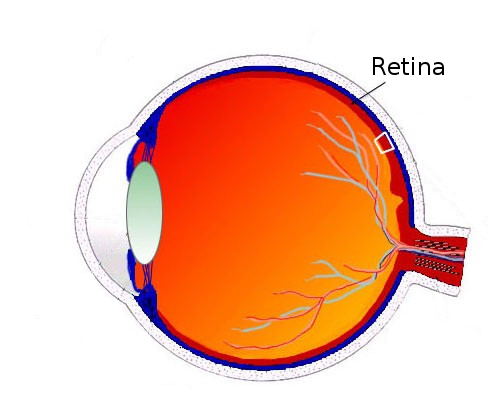
\includegraphics[width=\textwidth,valign=t]{Sagschem}
        \caption{Eye schematics}
        \label{eye-schematics}
      \end{subfigure}
      \begin{subfigure}[b]{0.32\textwidth}
          \centering
          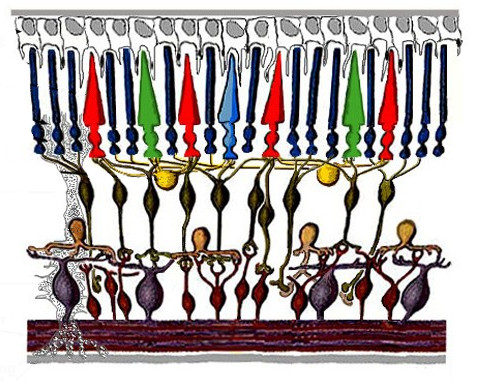
\includegraphics[width=\textwidth,valign=t]{schem}
          \caption{Retina}
          \label{retinal-layers}
      \end{subfigure}
      \begin{subfigure}[b]{0.3\textwidth}
          \centering
          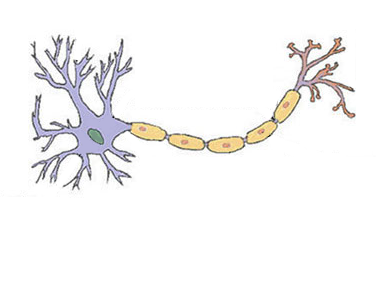
\includegraphics[width=\textwidth,valign=t]{Neuron-___-wikimedia-org}
          \caption{Neuron}
          \label{neuron}
      \end{subfigure}
            
    \caption{Anatomy of the (human) eye }
    \label{basic-eye-anatomy}
\end{figure}


Once the light enters the retina, it moves through several layers 
of neurons \cite{webvision} and hits the \emph{photoreceptors} 
(shown at the top of Fig. \ref{retinal-layers} \cite{wiki-images}). Light will 
elicit a chain reaction that has several steps, all occurring in 
the retina. On the central regions of the retinal layer there's a zone
called the \emph{Fovea}. The Fovea includes a small 
portion which is highly packed 
with \emph{cones} \cite{webvision-midget}, and has almost direct 
exposure to light, this region is known as the \emph{Foveal Pit}. 
This is the zone where images are acquired at the highest resolution.

The final step of the processing in the retina is carried out by 
\emph{ganglion cells} (bottom of Fig. \ref{retinal-layers}), 
this cells will emit spikes when certain 
conditions are met in the previous layers of the retina. The most
common type of cells are the \emph{Midget ganglion cells}. They 
are classified, depending on their input connectivity (dendritic
tree, left side of Fig. \ref{neuron}), as \emph{ON-centre} or 
\emph{OFF-centre} \cite{basab-thesis, webvision-midget}. 
What this means is that, an ON-centre cell will emit a spike
when the input in the ``centre'' region is stimulated but the 
surrounding area is not so much. The inverse case is true for 
OFF-centre type cells. The retina also contains another type
of ganglion cells whose dendritic trees span at much longer
distances, thus sampling wider portions of the image in the eye.
This last type of cells are called \emph{Parasol ganglion cells}
and come in both ON-centre and OFF-centre variants.






%\subsection{The foveal pit model}
%\label{sec-fov-pit}
%\begin{wrapfigure}{r}{0.5\textwidth}
    %\begin{figure}[hbt]
    \vspace{-20pt}
    \centering
    
\includegraphics[width=0.5\textwidth]{model-schematic}
    \caption{Schematic of the foveal pit model}
    \label{pic-fov-pit-model}
    %\end{figure}
\end{wrapfigure}

A functional model is one that treats a system as a black box
and tries to ``map'' observed inputs to their respective outputs 
by means of a set of mathematical expressions. The model created
by \citeauthor{basab-model} in \cite{basab-thesis, basab-model},
consists of several instances of four ganglion cells (midget and 
parasol, with ON and OFF centres) which transform the pixels in 
the received image into rank-ordered spike trains (Figure 
\ref{pic-fov-pit-model}). This model is based on previous work 
by \citeauthor{van-rullen-rate-coding} in
\cite{van-rullen-rate-coding}.


\subsubsection{Neural codes} There are many ways of encoding 
information using spikes. The most common one is rate-based, in 
which the average count of spikes fired by a neuron encodes a value. 
A different approach is to take the exact timing of spikes when 
they were generated as a means to transmit information. The latter 
has great encoding capabilities since there are many times in which 
a spike can occur. Rate-based codes tend to have limited 
representational power because the same spike count can happen due
to different inputs.

A simpler way of encoding spikes is to not really pretend to know 
exactly when they where actually emitted, but to just take into 
account the order in which they happened; this is referred as a 
rank-ordered encoding. This code has the advantage of being able 
to transmit more information than rate-based ones 
\cite{basab-thesis,thorpe-spike-rapid-processing, thorpe-rate-coding-theory}, 
yet maintain a simple way of interpretation. Furthermore, rank-ordered
encoding has shown to provide enough information for reconstruction
in about the highest 20 to 30\% spikes.


\subsubsection{Mathematical model} As discussed in section \ref{sec-retina},
the Foveal pit region of the retina is the highest resolution 
zone in the retina. This is taken into account by simulating one 
midget cell per pixel and one parasol cell about every 7 pixels.

Each ganglion cell is characterized by a Difference of Gaussian 
(DoG), described in equation \ref{eq-dog}. 

\begin{equation}
\label{eq-dog}
DoG_w(x,y) = \pm\frac{1}{2\pi\sigma_{w,c}^2}e^{\frac{-(x^2 + y^2)}{2\sigma_{w,c}^2}}
             \mp\frac{1}{2\pi\sigma_{w,s}^2}e^{\frac{-(x^2 + y^2)}{2\sigma_{w,s}^2}}
\end{equation}

where $\sigma_{w,c}$ and $\sigma_{w,s}$ are the standard deviation 
for the centre and surround components of the DoG at scale $w$ 
(cell type). The signs will be ($-$,$+$) if the 
ganglion cell is OFF-centre; ($+$,$-$) if it is ON-centre. The simulation 
of a cell is carried by a discrete convolution 
(Eq. \ref{eq-convolution}) of a DoG over the input image.

\begin{equation}
\label{eq-convolution}
C(x,y,w) = \sum_i \sum_j \left( I(i+x, j+y) \cdot DoG_w(i,j)\right)
\end{equation}

This will provide a set of coefficients $C$ for every scale $w$. 
The authors in \cite{van-rullen-rate-coding} refer to this as a 
wavelet-like transformation. The value of the coefficient will mean 
how soon does the neuron fire. If all $c_{i,w}$ are sorted according to their 
value, we shall posses a rank-ordered spikes set.\\

Cells are parametrized according to table \ref{tb-ganglion}. After
applying discrete convolutions to a test image Fig. \ref{pic-lena}, 
the results can be seen in Figs. \ref{pic-lena-M-OFF}, \ref{pic-lena-M-ON}
\ref{pic-lena-P-OFF} and \ref{pic-lena-P-ON}.

\begin{table}[hb]
    \caption{Simulation parameters for ganglion cells}
    \centering
\begin{TAB}(r,1em,1.5em){|c|c|c|c|c|}{|c|c|c|c|c|} 
    Cell type & Matrix size &  Centre std. dev. ($\sigma_c$) & 
    Surround std. dev. ($\sigma_s$)  & Sampling resolution  \\
    Midget OFF-centre  & $3 \times 3$ & $0.8$ & $6.7 \times \sigma_c$ &  col: 1, row: 1\\
    Midget ON-centre   & $11 \times 11$ & $1.04$ & $6.7 \times \sigma_c$ &  col: 1, row: 1\\
    Parasol OFF-centre & $61 \times 61$ & $8$ & $4.8 \times \sigma_c$ & col: 5, row: 3 \\
    Parasol ON-centre  & $243 \times 243$ & $10.4$ & $4.8 \times \sigma_c$ & col: 5, row: 3 \\
\end{TAB} 
\label{tb-ganglion}
\end{table}


\begin{figure}[hbt]
    \centering
    \begin{subfigure}[t]{0.15\textwidth}
        \centering
        \captionsetup{justification=centering,margin=0.1cm}
        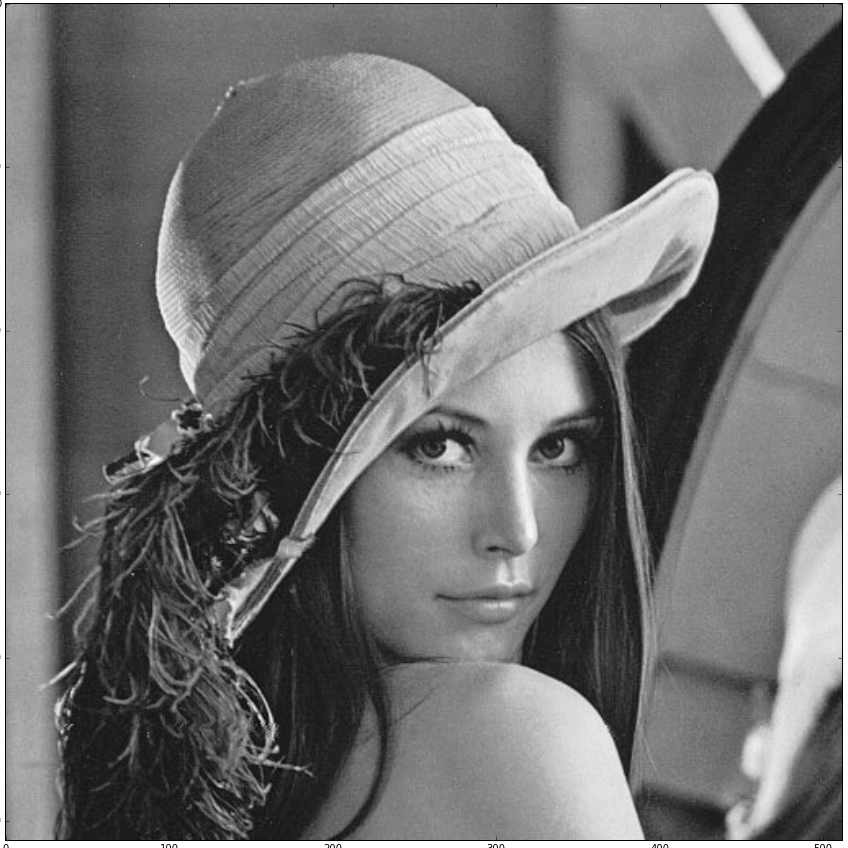
\includegraphics[width=\textwidth]{./Lena-gray}
        \caption{\\Original image}
        \label{pic-lena}
    \end{subfigure}
    \begin{subfigure}[t]{0.15\textwidth}
        \centering
        \captionsetup{justification=centering,margin=0.1cm}
        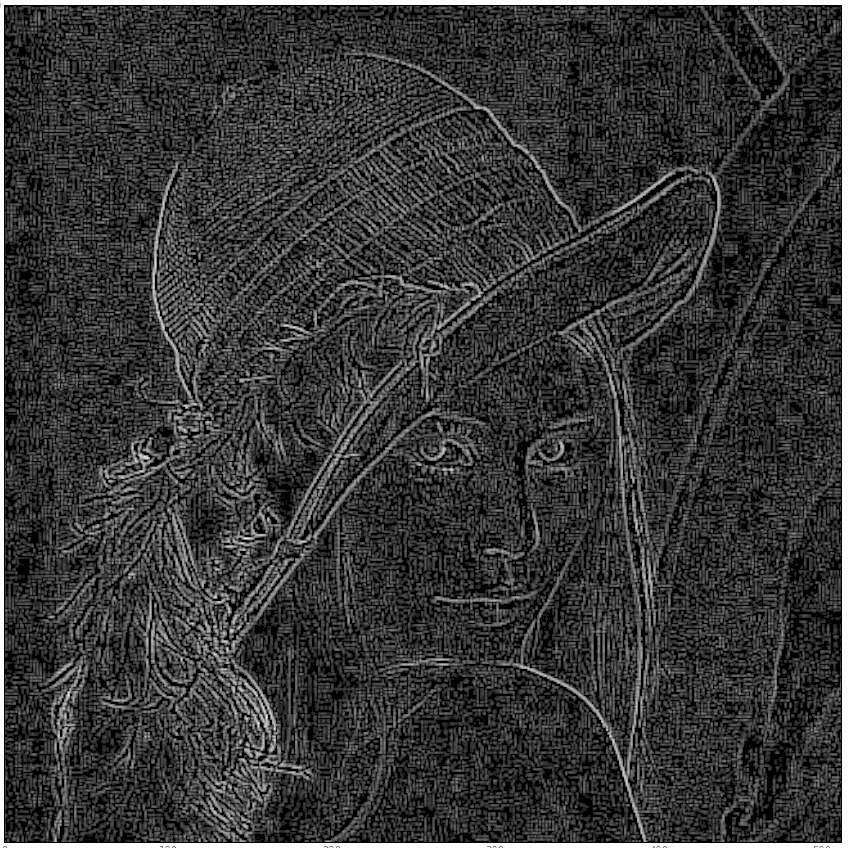
\includegraphics[width=\textwidth]{./Lena-midget_off}
        \caption{\\Midget OFF-centre}
        \label{pic-lena-M-OFF}
    \end{subfigure}
    \begin{subfigure}[t]{0.15\textwidth}
        \centering
        \captionsetup{justification=centering,margin=0.1cm}
        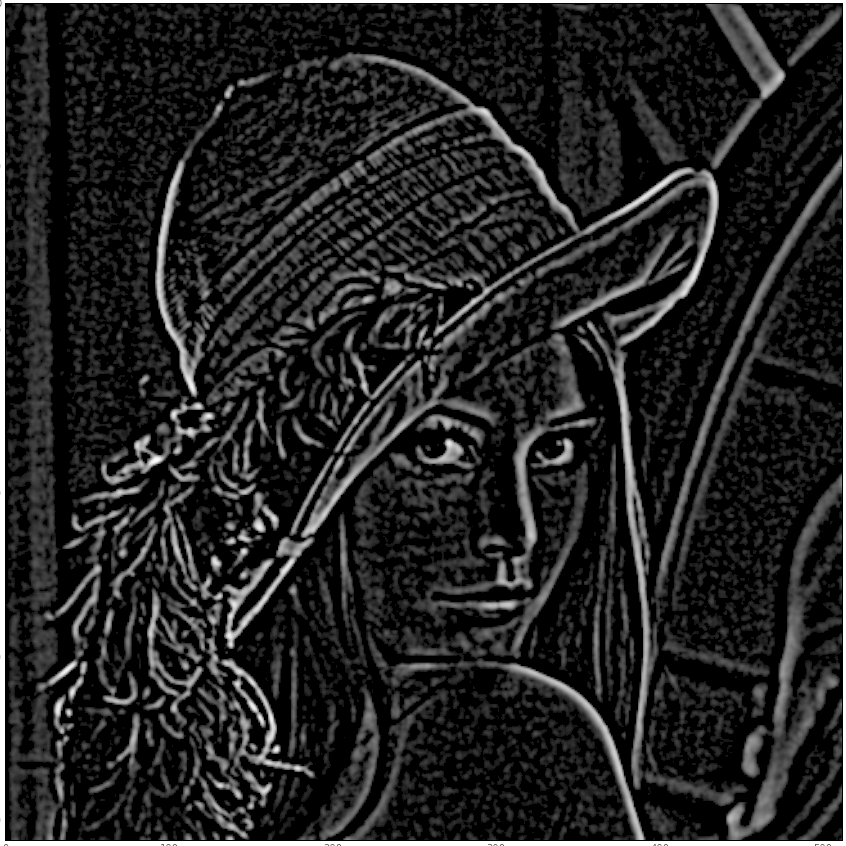
\includegraphics[width=\textwidth]{./Lena-midget_on}
        \caption{\\Midget ON-centre}
        \label{pic-lena-M-ON}
    \end{subfigure}
    \begin{subfigure}[t]{0.15\textwidth}
        \centering
        \captionsetup{justification=centering,margin=0.1cm}
        
\includegraphics[width=\textwidth]{./Lena-parasol_off}
        \caption{\\Parasol OFF-centre}
        \label{pic-lena-P-OFF}
    \end{subfigure}
    \begin{subfigure}[t]{0.15\textwidth}
        \centering
        \captionsetup{justification=centering,margin=0.1cm}
        
\includegraphics[width=\textwidth]{./Lena-parasol_on}
        \caption{\\Parasol ON-centre}
        \label{pic-lena-P-ON}
    \end{subfigure}
    \caption{Results of simulating ganglion cells (convoluted images, enhanced for better contrast)}
\end{figure}

%\subsection{Parallel implementation}
%\label{sec-parallel}
%The retinal model described in section \ref{sec-fov-pit} is
parallel in nature it involves changing each pixel locally.
Convolution kernels are computed and stored in memory prior 
to any convolution procedure. OpenCL is used since 
the same code can be used in multiple Operating Systems (OS) 
and hardware targets \cite{munshi2011opencl}.

\subsection{Na\"{i}ve approach}
\begin{wrapfigure}{r}{0.55\textwidth}
    \vspace{-26pt}
    \begin{minipage}{0.55\textwidth}
        \begin{pseudocode}{Na\"ive convolution}{image \; I,\; kernel\; K}
            \label{code-naive-convolution}
            \FOREACH pixel\; p \in I \DO \textrm{(in parallel):}\\
            \hspace{0.7cm} x \GETS row(p), \; y \GETS column(p),\; sum \GETS 0,\; k \GETS 0\\
            \hspace{0.7cm} \FOR i \GETS x - width(K)/2 \TO x + width(K)/2 \\
            \hspace{1.4cm} \FOR j \GETS y - width(K)/2 \TO y + width(K)/2 \\
            \hspace{2.1cm} sum \GETS value(I,i,j)*value(K,k),\; k \GETS k + 1 \\
            \hspace{0.7cm} \RETURN {convolved\_image \GETS pixel(sum,x,y) }\\
        \end{pseudocode}
    \vspace*{-25pt}
    \end{minipage}
    \vspace*{-0.7cm}
\end{wrapfigure}

The easiest way of implementing the ganglion cell simulation
is to code equation \ref{eq-convolution} into OpenCL and do
the same operation for every pixel in the image (code). This is a
rather inefficient way of performing convolution on images 
\cite{cmsoft-opencl, reda-opencl}. \\

\subsection{Coding optimization}
The first aspect to consider in optimizing code 
\ref{code-naive-convolution} is that not every pixel in the 
image will have valid data to compute a convolution, thus we'll 
discard them. Without having to worry about valid or invalid 
pixels, one can easily unroll the two inner $\FOR$ loops in 
code \ref{code-naive-convolution} and
free the processors from those operations. The next thing to notice
is that both the image ($I$) and convolution kernel ($K$) may
be stored in local (\emph{faster}, shared by a set of processors) 
memory instead of global (\emph{slower}, shared by \emph{all} 
cores). Changing data access from global to local memory brings
a significant speed-up.

\subsubsection{Separability}
The kernel that represents the DoG is not separable, i.e. 
it may not be computed by the multiplication of a column and
a row vector. Nonetheless the matrices that, when subtracted, 
form a DoG are, in fact, separable (Eq. \ref{eq-separable}). 

\begin{align}
C(x,y,w) &= \sum_i \sum_j \left( \left[
              \pm\frac{1}{2\pi\sigma_{w,c}^2}
                  e^{\frac{-(i^2 + j^2)}{2\sigma_{w,c}^2}}
              \mp\frac{1}{2\pi\sigma_{w,s}^2}
                  e^{\frac{-(i^2 + j^2)}{2\sigma_{w,s}^2}} \right]
              I(i+x, j+y) 
            \right) \\
         &= \pm\left[\frac{1}{2\pi\sigma_{w,c}^2} 
                     \sum_i e^{\frac{-i^2}{2\sigma_{w,c}^2}} 
                     \sum_j e^{\frac{-j^2}{2\sigma_{w,c}^2}}
                     I(i+x, j+y)
                \right]_{c} %\nonumber\\
             \mp \left[ \frac{1}{2\pi\sigma_{w,s}^2}
                        \sum_i e^{\frac{-i^2}{2\sigma_{w,s}^2}}
                        \sum_j e^{\frac{-j^2)}{2\sigma_{w,s}^2}}
                        I(i+x, j+y) 
               \right]_{s}
\label{eq-separable}
\end{align}

We take advantage of this to perform a \emph{separable convolution}; 
the first step is to convolve the image with a horizontal kernel, 
next we take the resulting image and convolve it vertically. This 
reduces the computation and memory requirements from $O(N*M)$ to $O(N+M)$.

\subsubsection{Tiled convolution}

\begin{wrapfigure}{r}{0.55\textwidth}
    \centering
    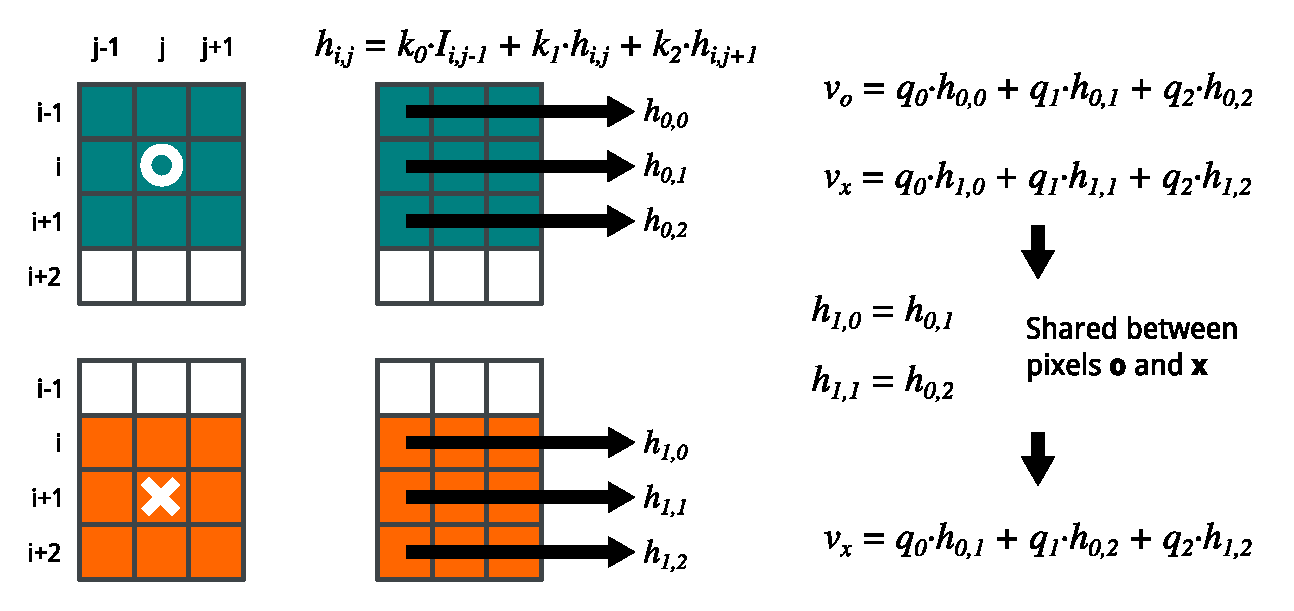
\includegraphics[width=0.55\textwidth]{tiled-conv}
    \caption{Tiled convolution flow}
    \label{pic-tiled-conv}
\end{wrapfigure}


The final step is an optimization published by Advanced Micro Devices (AMD) 
described in \cite{tiled-convolution}. They take advantage from using
separable kernels and reusing operations to get the most out of resources.
We can see separable convolution as a two step process. 
First a horizontal convolution step that creates a set of coefficients 
($h_{y,x}$ in the middle of Fig. \ref{pic-tiled-conv}). Most $h$ coefficients 
are shared by immediate vertical neighbours (e.g. pixels $\hm{\circ}$ 
and $\bm{\times}$ in Fig. \ref{pic-tiled-conv}), thus it is desired 
to reuse them instead of re-computing them. This way, every core in the GPU 
will compute 2 pixels in order to efficiently compute a 2D convolution; plus 
most of this operations are done using registers which is the fastest memory 
available to the cores.


\subsubsection{Comparison}
The Naïve approach seems to be much faster than any other attempts for the 
smallest kernel ($3\times3$), this is simply because a single DoG kernel would
require 9 operations while a separated DoG requires 12. As the size of the
kernels increases tiled convolution has the lead performance-wise.
\begin{table}[hbt]
    \begin{center}
        \caption{Time comparison of different convolution algorithms.}
        \bgroup
        \def\arraystretch{1.2}
        \begin{tabular}{|c|c|c|c|c|}
            \hline Algorithm & Midget Off-centre & Midget On-centre & Parasol Off-centre & Parasol On-centre \\
            \hline Naïve     & 0.000932 s & 0.003150 s & 0.058797 s & N/A\footnote{Unable to fit kernel into constant memory.} \\ 
            \hline Separated & 0.002953 s & 0.005550 s & 0.017261 s & 0.047226 s \\ 
            \hline Tiled     & 0.001947 s & 0.002722 s &  & \\ 
            \hline 
        \end{tabular} 
        \egroup
    \end{center}
\end{table}
\vspace*{-20pt}

For the final implementation we take the best times for every \emph{cell type}
and combine them into a ``convolution'' object under the Python programming language.
%\subsection{Lateral inhibition}
%\label{sec-reconstruction}
%The problem of environment reconstruction implies taking a collection of sensed data and transforming it into a representation of the scenes the data was taken from (Figure~\ref{fig:slam:example}). This work will focus in getting a three-dimensional reconstruction from sensor data. The most studied types of sensed data are depth (e.g. laser radar, sonar) and visual (e.g. photography, video). For our research the main input will be visual, either from video sources converted into spikes or a DVS. 

\begin{figure}[h]
  \begin{center}
    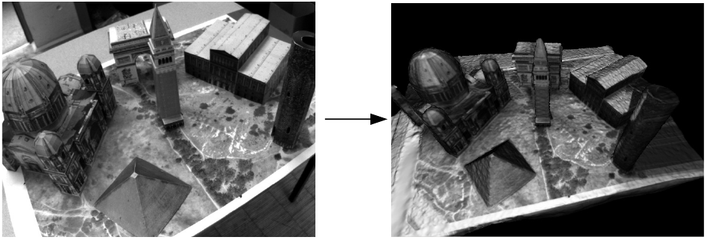
\includegraphics[width=0.8\textwidth]{live-cam}
    \caption{Dense 3D reconstruction. Left: camera input; right: reconstruction. Adapted from~\cite{livecam}}
    \label{fig:slam:example}
  \end{center}
\end{figure}

\section{Simultaneous localization and mapping}
Environment reconstruction has been receiving a lot of attention from the research  community, specially using Simultaneous Localization and Mapping (SLAM) procedures. 
Can be categorized according to the problem methodology in Extended Kalman filters, graph-based optimization and particle filters~\cite{Thrun2008_SLAM}.
The first work that used an incremental map building was done by \citeauthor{smith1990estimating}~\cite{smith1990estimating}, where the authors used Extended Kalman Filters (EKF) to recursively estimate a vector that includes the location of the sensing entity and feature elements of the environment. The uncertainty of the elements is modelled using probability density functions. Disadvantages of this approach is that the EKF procedure my be thrown off by incorrect measurements and it's limited to few landmarks.

The first solution using a graph-based optimization technique was presented by \citeauthor{lu1997globally}~\cite{lu1997globally}. The position of the entity and landmarks in the environment are represented as nodes in a graph. As the robot moves or senses landmarks, it adds nodes which are connected by arcs. Consecutive locations are tied together and landmarks are associated to the locations they were sensed in. If the graph is seen as a mass-spring system, the solution comes from the minimal energy state of the system. The main disadvantage of this methodology is that most implementations use off-line optimization of the graph, but it's able to keep track of up to $10^8$ landmarks~\cite{Thrun2008_SLAM}. 

The third common approach to the SLAM problem is using particle filters, it was first introduced by \citeauthor{montemerlo2002fastslam}~\cite{montemerlo2002fastslam}. Each particle is thought of as a guess for the trajectory of the entity in the environment. These particles are generated and, if degraded, re-sampled. An issue that has been noted for this method is that the complexity depends on the number of particles and the number of landmarks, this leads to a huge representation of the mapping; and there is no way of knowing how many particles are needed. 

A classification can be made by the nature of the sensing devices. While the SLAM problem with depth data may be considered closed, solving it with visual input alone is still an open research question. Furthermore, achieving a solution with spiking neural networks has received little attention despite the efficiency that this approach could provide. Most SLAM solutions only handle static indoor environments, although the vast majority of the world is outdoors and inherently dynamic. Another open question is how to deal with continuously accumulating sensing and/or inference errors, the recovery from which is key for dealing with ever-changing environments. 
%Papers that summarize and explain the mathematical framework of the SLAM problem can be found in the references chapter~\cite{Thrun2008_SLAM,Fuentes-Pacheco2012-slam,durrant2006simultaneous,bailey2006simultaneous}. 

In terms of sensor input, a division of SLAM that uses visual information as the sole external input is, not surprisingly, called \emph{visualSLAM}. In that group of algorithms  there are some that use a single camera, binocular vision, DVS, or RGB-D cameras, to name a few (Figure~\ref{fig:slam:camera-comparison}). 

A conventional camera captures colour information available for a fixed period of time (i.e. a frame). An RGB-D camera captures both colour and depth information; the latter is usually done with laser radars or structured light. A DVS is a visual sensor that emits an event whenever (i.e. dynamically) a pixel senses a change in contrast over time. A benefit of this is that static objects in a scene have a low probability of generating an event.
%The latter is not using only visual information, but it is using just a camera. 

\begin{figure}[h]
  \begin{center}
    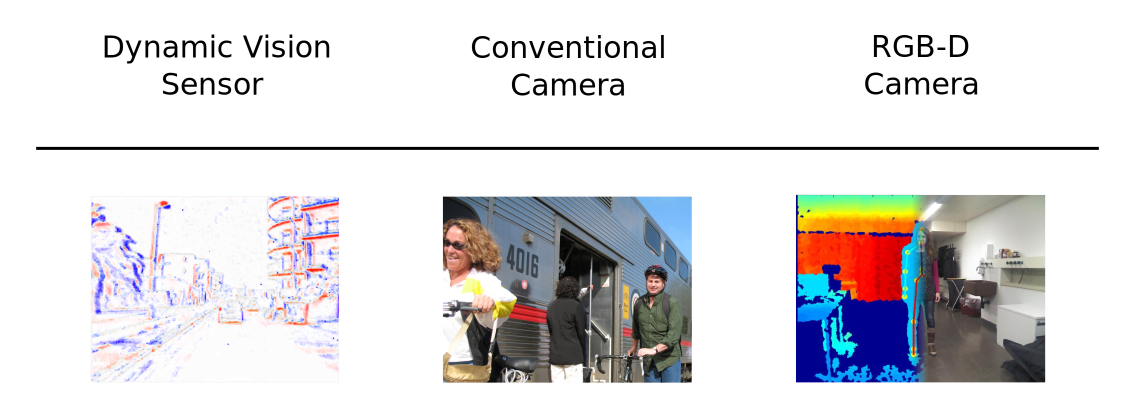
\includegraphics[width=\textwidth]{camera-comparison}
    \caption{Comparison of different visual inputs. Left: a DVS sensor, captures temporal contrast changes in a $\mu s$ scale (red and blue colours). Middle: a conventional camera captures light accumulated during a time window. Right: an RGB-D camera provides depth (left half of the sample image) plus colour (right half) information of a scene.}
    \label{fig:slam:camera-comparison}
  \end{center}
\end{figure}


If only images are used, the correspondence problem arises; where is a feature from one frame located in the next. To solve this, there are mainly two efficient approaches: the first is to use descriptors~\cite{lowe1999object,bay2006surf,alahi2012freak} (i.e. salient features of objects) or to use landmarks~\cite{sola2012impact,frintrop2006attentional} (i.e. full objects, often artificial). In our approach, the use of visual landmarks is chosen due to neural networks' image recognition capabilities. 

The algorithm known as \emph{MonoSLAM}~\cite{davison2007monoslam}, was the first to solve the SLAM problem in real time with a single camera. It is able to perform at 30 frames per second and considers both position and orientation of the camera. The limitations of this work is that is confined to indoor environments and it models motion with constant velocities.

%Spiking neural networks (SNN) need to convert any visual input to spike trains. 
\emph{Event-based 3D SLAM}~\cite{Weikersdorfer2014} is a work that uses a DVS  with RGB-D camera to create a sparse representation of 3D frames. It then uses Bayesian network and condensation particle filter algorithm. They obtain good results with few resources, but they are not using ANNs.

\citeauthor{villaverde2006morphological}~\cite{villaverde2006morphological} report a neural network approach for solving the localization and mapping. An interesting point is the use of Morphological Associative Memories (MAM), which are a type of content-addressable memory that uses morphological operations (dilation and erosion). In the learning and retrieval stages, MAMs utilize sums instead of products, and minimum (erosion) or maximums (dilation) instead of sums for vector and matrix operations. The main advantage to use MAMs is that they can store and recall morphologically strong-independent patterns, which have been proven to be robust against noise. 

Neural networks have also been used to complement other SLAM solutions, for instance by using a NN to better estimate the mapping in presence of noise and errors~\cite{choi2007neural}. A one hidden layer perceptron is used to estimate the uncertainty of the model and increase its accuracy. Another interesting NN extension to SLAM algorithms was reported by \citeauthor{saeedi2011neural}~\cite{saeedi2011neural}, they use a neural network to fuse the results of SLAM algorithms performed by multiple robots. The NN cluster representations into an occupancy grid map.

Hippocampus-based navigation studies has been developed by the neuroscience community. A simulation of a model of place cells is tested in a small robot through neural networks~\cite{burgess1997robotic}, with good results in terms of self-localization and environment recognition. A review of the different aspects of the theory behind hippocampus navigation was published by \citeauthor{sunderhauf2010learning}~\cite{sunderhauf2010learning}. 

A bio-inspired algorithm to solve the SLAM problem is \emph{RatSLAM}, it's based on the hippocampus of rodents, which has been studied for its involvement in navigation tasks. Pose is estimated by activity of place cells arranged in a competitive attractor neural network. If visual information is familiar with respect to a place cell, the latter gets excitatory input. Odometry helps select current active place cells. Results in semi-Cartesian space, on-line incremental, distributed representation via place cells~\cite{rat-slam,milford2008robot}.


\section{Proposal}
Our approach to solve the SLAM problem is to use spiking neural networks for their efficiency and biological plausibility. The primary external sensor would be visual, either a conventional camera or a dynamic vision sensor. The information from the sensor would then be scanned for landmarks (e.g. a lamp, door, tree, stop sign). To infer the position of the viewer, we will look for inspiration on published work that uses hippocampus models as that organ is known to be a basic component for navigational tasks in animals (see Section~\ref{sec:brain:hippo}). A link from visual information to the structure created through the neural network will have to be developed; from this link, a full 3D reconstruction should be available.\\

The milestones of this project are:
\begin{enumerate}
  \item Landmark identification and recognition through spike-based visual input. The initial task would be to develop an on-line learning neural network, the latter would then be modified for identification and recognition tasks.
  \item Tracking of landmarks. Adapt the network from the previous step to be able to provide information of where the landmarks are; this might include some attention modulation for moving objects.
  \item Localization estimation and depth perception. From the information provided by the tracking network (and possibly other sensors), feed another part of a larger network that will estimate the localization of the viewer. A result from this estimation would be the ability to perceive the distance of objects in the scene. 
  \item Mapping and reconstruction. The mapping problem will be solved in parallel to the localization one. For reconstruction a way to connect acquired visual information (i.e. video frames) to the estimated structure in the neural network will be developed and, thus, a full 3D reconstruction achieved.
\end{enumerate}


\section{Conclusions}
A complete model the visual cortex remains an open research question. Though many neural networks and computer vision models account for single visual functions, a unified solution has not been developed. Since environment reconstruction makes use of many of these functions, this research could lead to contributions to a general theory of vision. 

A hierarchical neural networks approach promises to have better results. The training of deep spiking neural networks is still in early stages of research, which brings another opportunity for contributions to neuroscience. Recurrent neural networks could provide the necessary framework to solve the training problem.
%\clearpage



\section{Project Plan}
\label{sec-project-plan}
%\hspace*{10cm}     
\begin{figure}[htbp]
  \begin{center}
    \begin{rotate}{270}

      \begin{ganttchart}[x unit = 5mm,
                         y unit chart = 5.6mm,
                         vgrid={*1{themecolor, dotted}},
                         compress calendar, 
                         time slot format=isodate-yearmonth,
                         title/.append style={draw=none, fill=themecolordark},
                         title label font=\sffamily\bfseries\color{white},
                         title label node/.append style={below=-1.6ex},
                         title left shift=.05,
                         title right shift=-.05,
                         title height=1]{2014-09}{2017-08}
        \gantttitlecalendar{year, month} \\
         \ganttbar{Learn background concepts}{2014-09}{2015-02}\\
         \ganttbar{Implement retinal models}{2014-12}{2015-04}\\
         \ganttbar{Familiarize with SpiNNaker}{2015-01}{2015-08}\\
         \ganttbar{Develop learning algorithms}{2015-07}{2016-04}\\
         \ganttbar{Develop classification networks}{2015-10}{2016-08}\\
         \ganttbar{Develop vision algorithms}{2016-08}{2017-04}\\
         \ganttbar{Theses writing}{2016-10}{2017-08}
      \end{ganttchart}

    \end{rotate}
  \end{center}
\end{figure}




%\end{multicols}

\end{document}
